%-------------------------------------------------------------------------------%
%	PACKAGES AND OTHER DOCUMENT CONFIGURATIONS
%-------------------------------------------------------------------------------%

\documentclass[final]{beamer}

\usepackage[scale=1.24]{beamerposter} % Use the beamerposter package for laying out the poster

%\usetheme{confposter} % Use the confposter theme supplied with this template
\usetheme[faculty=chemo]{fibeamer}

%\setbeamercolor{block title}{fg=ngreen,bg=white} % Colors of the block titles
%\setbeamercolor{block body}{fg=black,bg=white} % Colors of the body of blocks
%\setbeamercolor{block alerted title}{fg=white,bg=dblue!70} % Colors of the highlighted block titles
%\setbeamercolor{block alerted body}{fg=black,bg=dblue!10} % Colors of the body of highlighted blocks
% Many more colors are available for use in beamerthemeconfposter.sty
%-----------------------------------------------------------
% Define the column widths and overall poster size
% To set effective sepwid, onecolwid and twocolwid values, first choose how many columns you want and how much separation you want between columns
% In this template, the separation width chosen is 0.024 of the paper width and a 4-column layout
% onecolwid should therefore be (1-(# of columns+1)*sepwid)/# of columns e.g. (1-(4+1)*0.024)/4 = 0.22
% Set twocolwid to be (2*onecolwid)+sepwid = 0.464
% Set threecolwid to be (3*onecolwid)+2*sepwid = 0.708

\newlength{\sepwid}
\newlength{\onecolwid}
\newlength{\twocolwid}
\newlength{\threecolwid}
\setlength{\paperwidth}{46.8in} % A0 width: 46.8in
\setlength{\paperheight}{33.1in} % A0 height: 33.1in
\setlength{\sepwid}{0.024\paperwidth} % Separation width (white space) between columns
\setlength{\onecolwid}{0.21\paperwidth} % Width of one column
\setlength{\twocolwid}{0.451\paperwidth} % Width of two columns
\setlength{\threecolwid}{0.678\paperwidth} % Width of three columns
%\setlength{\topmargin}{-0.5in} % Reduce the top margin size
%-----------------------------------------------------------

\usepackage{graphicx}  % Required for including images
\usepackage{booktabs} % Top and bottom rules for tables

%-------------------------------------------------------------------------------%
%	TITLE SECTION 
%-------------------------------------------------------------------------------%

\title{Deep Learning for the Internet of Things with Edge Computing} % Poster title

\author{He Li, Kaoru Ota, and Mianxiong Dong} % Author(s)

\institute{Research Fund for Postdoctoral Program of Muroran Institute of Technology - KDDI Foundation} % Institution(s)

%-------------------------------------------------------------------------------%

\begin{document}
\addtobeamertemplate{block end}{}{\vspace*{2ex}} % White space under blocks
\addtobeamertemplate{block example end}{}{\vspace*{2ex}} % White space under example blocks
\addtobeamertemplate{block alerted end}{}{\vspace*{2ex}} % White space under highlighted (alert) blocks

\setlength{\belowcaptionskip}{2ex} % White space under figures
\setlength\belowdisplayshortskip{2ex} % White space under equations
%\begin{darkframes} % Uncomment for dark theme, don't forget to \end{darkframes}
\begin{frame} % The whole poster is enclosed in one beamer frame

%==========================Begin Head===============================
  \begin{columns}
   \begin{column}{0.9\linewidth}
    \vskip1cm
    \centering
    \usebeamercolor{title in headline}{\color{fg}\Huge{\textbf{\inserttitle}}\\[0.5ex]}
    \usebeamercolor{author in headline}{\color{fg}\Large{\insertauthor}\\[1ex]}
    \usebeamercolor{institute in headline}{\color{fg}\large{\insertinstitute}\\[1ex]}
    \vskip1cm
   \end{column}
   \begin{column}{0.1\textwidth}
   
\includegraphics[scale=4]{Resources/Logo_UNIS.png}
   \end{column}
   \vspace{1cm}
  \end{columns}
 \vspace{1cm}

%==========================End Head===============================

\begin{columns}[t] % The whole poster consists of three major columns, the second of which is split into two columns twice - the [t] option aligns each column's content to the top

\begin{column}{\sepwid}\end{column} % Empty spacer column

\begin{column}{\onecolwid} % The first column

%-------------------------------------------------------------------------------%
%	OBJECTIVES
%-------------------------------------------------------------------------------%

\begin{exampleblock}{Objectives}

\begin{itemize}
\item Introduce deep learning for IoTs into the edge computing environment.
\item Design a novel offloading strategy to optimize the performance of IoT deep learning applications with edge computing.
\item Test the performance of executing multiple deep learning tasks in an edge computing environment with our strategy.  
%\item Show that our method outperforms other optimization solutions on deep learning for IoT.
\end{itemize}

\end{exampleblock}

%-------------------------------------------------------------------------------%
%	INTRODUCTION
%-------------------------------------------------------------------------------%

\begin{exampleblock}{Introduction}

We introduce deep learning for IoT into the edge computing environment to improve learning performance as well as to reduce network traffic. We formulate an elastic model that is compatible with different deep learning models. We state a scheduling problem to maximize the number of deep learning tasks with the limited network bandwidth and service capability of edge nodes. We design offline and online scheduling algorithms to solve the problem. We perform extensive simulations with multiple deep learning tasks and given edge computing settings.

%This statement requires citation \cite{Smith:2012qr}.

\end{exampleblock}

%------------------------------------------------

\begin{figure}
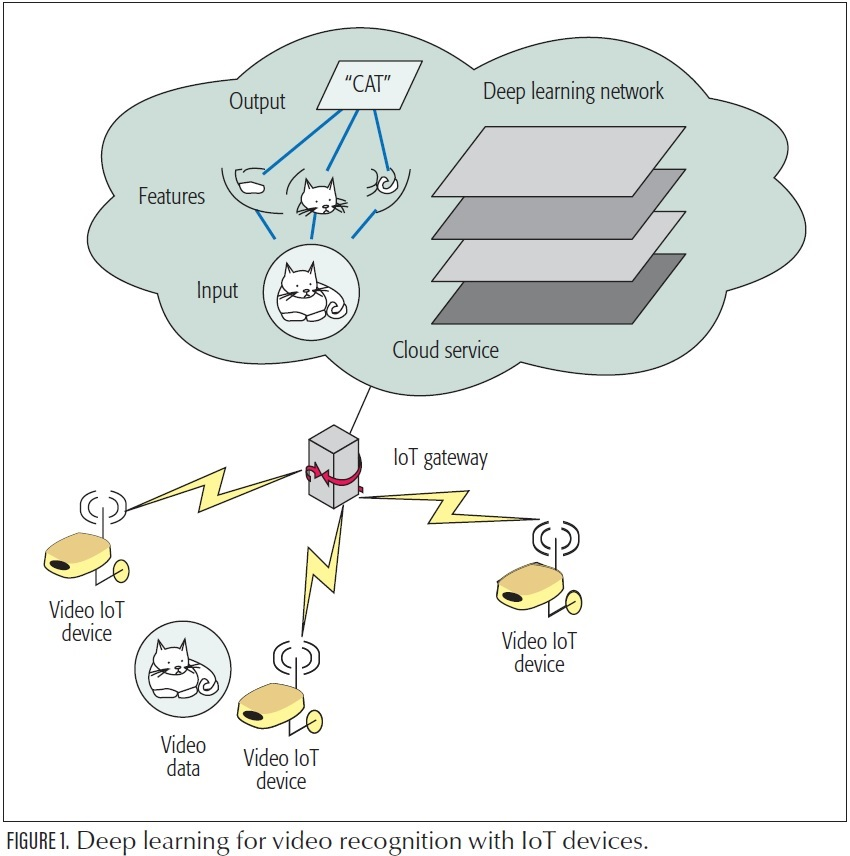
\includegraphics[width=0.8\linewidth]{Resources/Figura-1.jpg}
%\caption{Figure caption}
\end{figure}

%-------------------------------------------------------------------------------%

\end{column} % End of the first column

\begin{column}{\sepwid}\end{column} % Empty spacer column

\begin{column}{\twocolwid} % Begin a column which is two columns wide (column 2)

\begin{columns}[t,totalwidth=\twocolwid] % Split up the two columns wide column

\begin{column}{\onecolwid}\vspace{-.74in} % The first column within column 2 (column 2.1)

%-------------------------------------------------------------------------------%
%	MATERIALS
%-------------------------------------------------------------------------------%

\begin{exampleblock}{Deep Learning and Edge Computing}

Edge computing is proposed to move computing ability from centralized cloud servers to edge nodes near the user end. Edge computing brings two major improvements to the existing cloud computing. The first one is that edge nodes can preprocess large amounts of data before transferring them to the central servers in the cloud. The other one is that the cloud resources are optimized
by enabling edge nodes with computing ability.
\begin{figure}
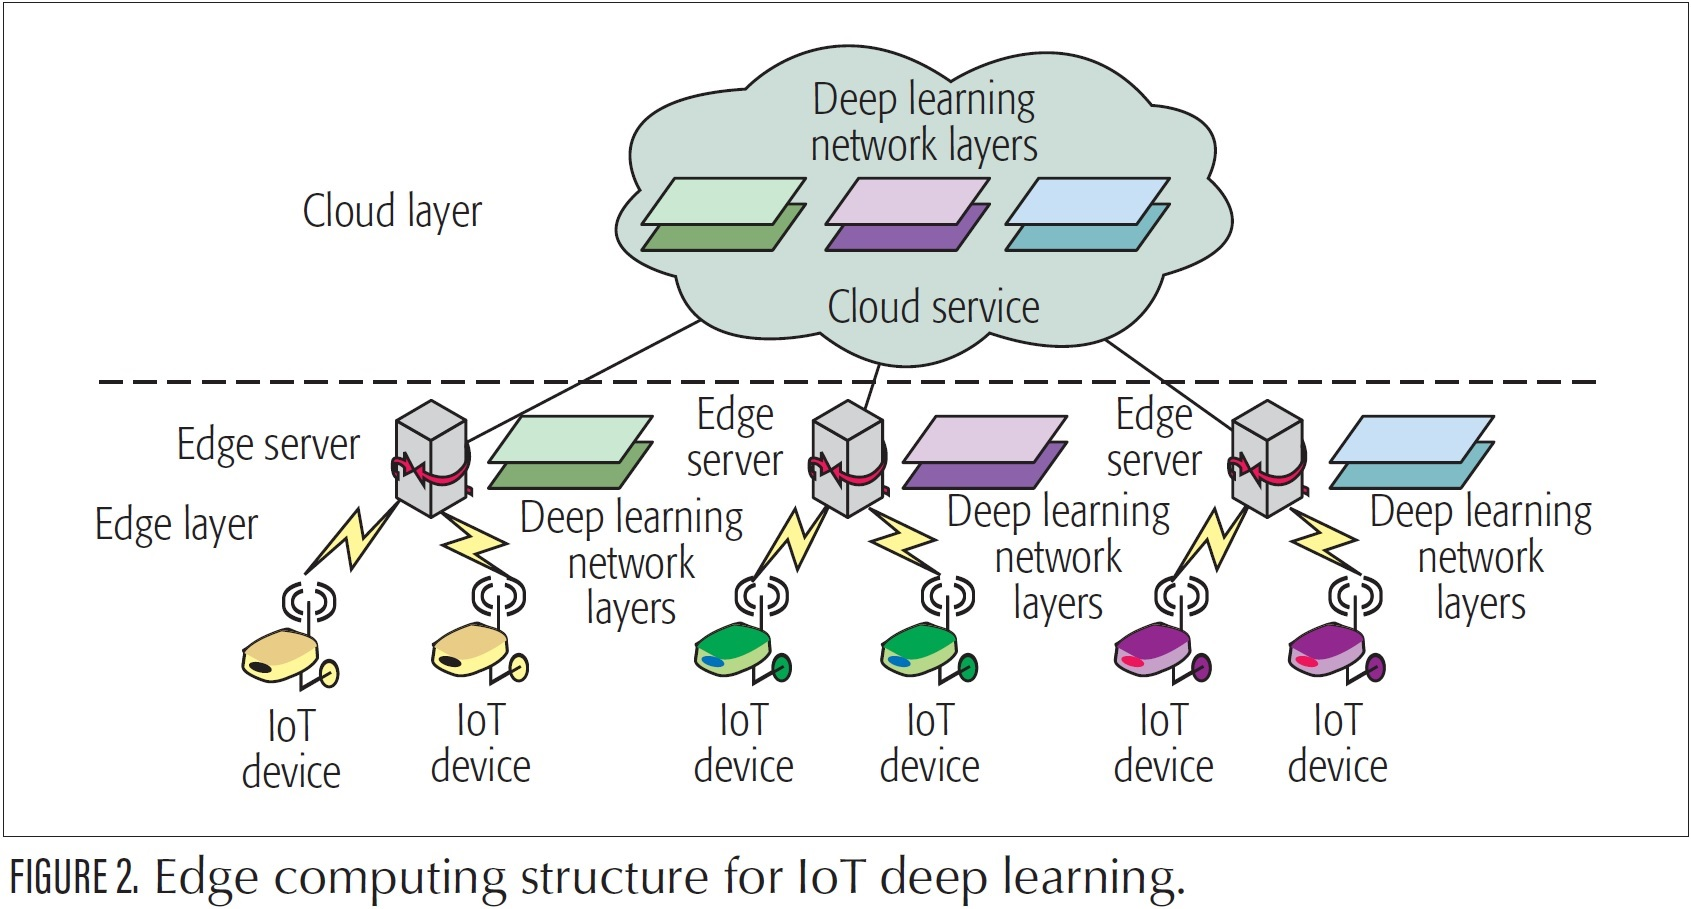
\includegraphics[width=1\linewidth]{Resources/Figura-2.jpg}
%\caption{Figure caption}
\end{figure}

\end{exampleblock}

%-------------------------------------------------------------------------------%

\end{column} % End of column 2.1
\begin{column}{\sepwid}\end{column} % Empty spacer column

\begin{column}{\onecolwid}\vspace{-.74in} % The second column within column 2 (column 2.2)

%-------------------------------------------------------------------------------%
%	METHODS
%-------------------------------------------------------------------------------%

\begin{exampleblock}{Deep Learning IoT in Edge Computing}

The structure for IoT deep learning tasks, consists of two layers as well as a typical edge computing structure. In the edge layer, edge servers are deployed in IoT gateways for processing collected data. We first train the networks in the cloud server. After the training, we divide the learning networks. One part includes the lower layers near the input data, while another part includes the higher layers near the output data. We deploy lower layers into edge servers and higher layers into the cloud for offloading processing. The collected data are input into the first layer in the edge servers. The edge servers load the intermediate data from the lower layers and then transferred data to the cloud server as the input data for the higher layers.

\end{exampleblock}

%-------------------------------------------------------------------------------%

\end{column} % End of column 2.2

\end{columns} % End of the split of column 2 - any content after this will now take up 2 columns width

%-------------------------------------------------------------------------------%
%	IMPORTANT RESULT
%-------------------------------------------------------------------------------%

\begin{alertblock}{Important Result}

The most important benefit of deep learning over machine learning is the better performance with large data scale since many IoT applications generate a large amount of data for processing. Another benefit is that deep learning can extract new features automatically for different problems.

\end{alertblock} 

%-------------------------------------------------------------------------------%

\begin{columns}[t,totalwidth=\twocolwid] % Split up the two columns wide column again

\begin{column}{\onecolwid} % The first column within column 2 (column 2.1)

%-------------------------------------------------------------------------------%
%	MATHEMATICAL SECTION
%-------------------------------------------------------------------------------%

\begin{exampleblock}{Scheduling Problem and Solution}
To assign maximum tasks in the edge computing structure by deploying deep learning layers in IoT edge servers such that the required transferring latency of each task can be guaranteed, denoted by

\begin{columns}
\begin{column}{0.5\linewidth}
\begin{align}
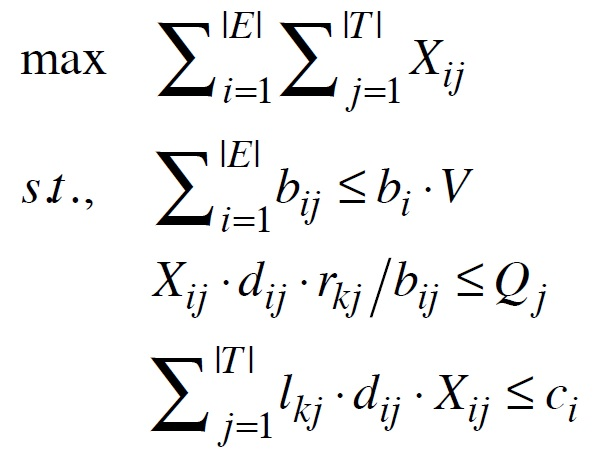
\includegraphics[width=0.8\linewidth]{Resources/Equation.jpg}
\end{align}
\end{column}
\begin{column}{0.5\textwidth}
\\
where Xij = 1 if task tj is deployed in edge server ei; otherwise, Xij = 0.
\end{column}
\end{columns}

\end{exampleblock}

%-------------------------------------------------------------------------------%

\end{column} % End of column 2.1
\begin{column}{\sepwid}\end{column} % Empty spacer column

\begin{column}{\onecolwid} % The second column within column 2 (column 2.2)

%-------------------------------------------------------------------------------%
%	RESULTS
%-------------------------------------------------------------------------------%

\begin{exampleblock}{Performance Evaluation}

\begin{figure}
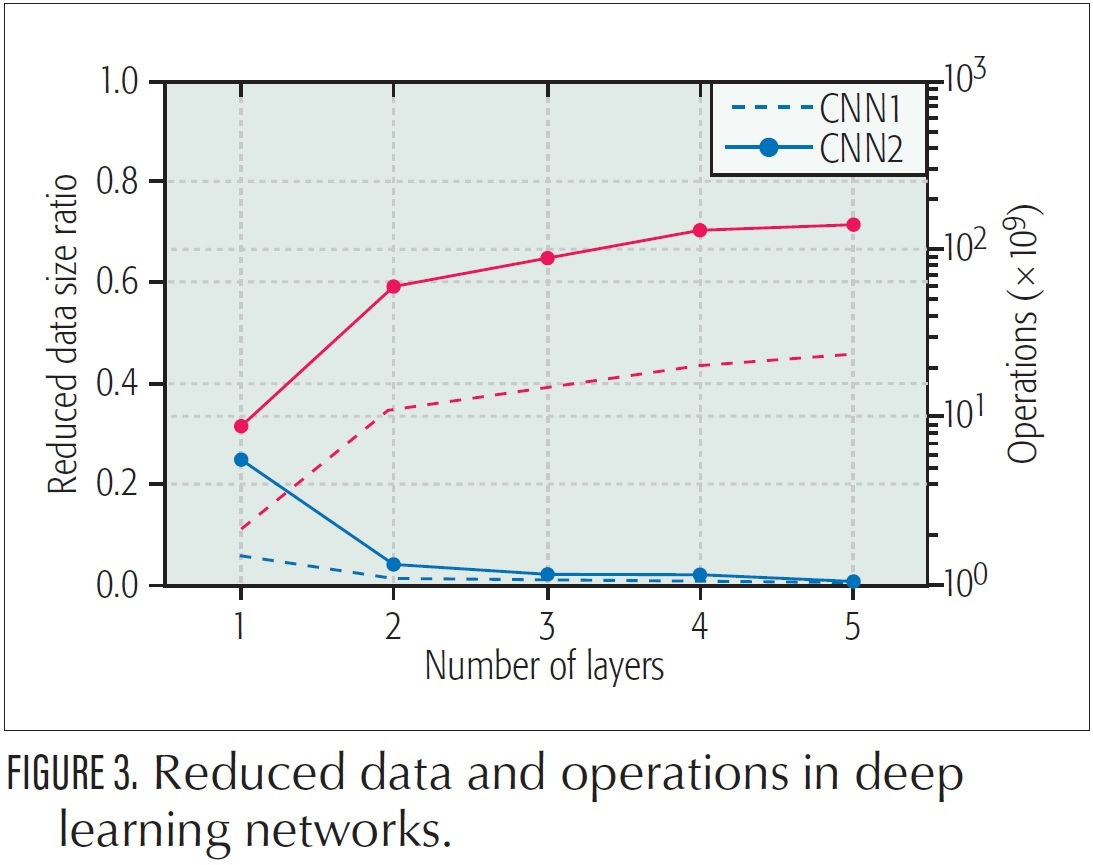
\includegraphics[width=0.9\linewidth]{Resources/Figura-3.jpg}
%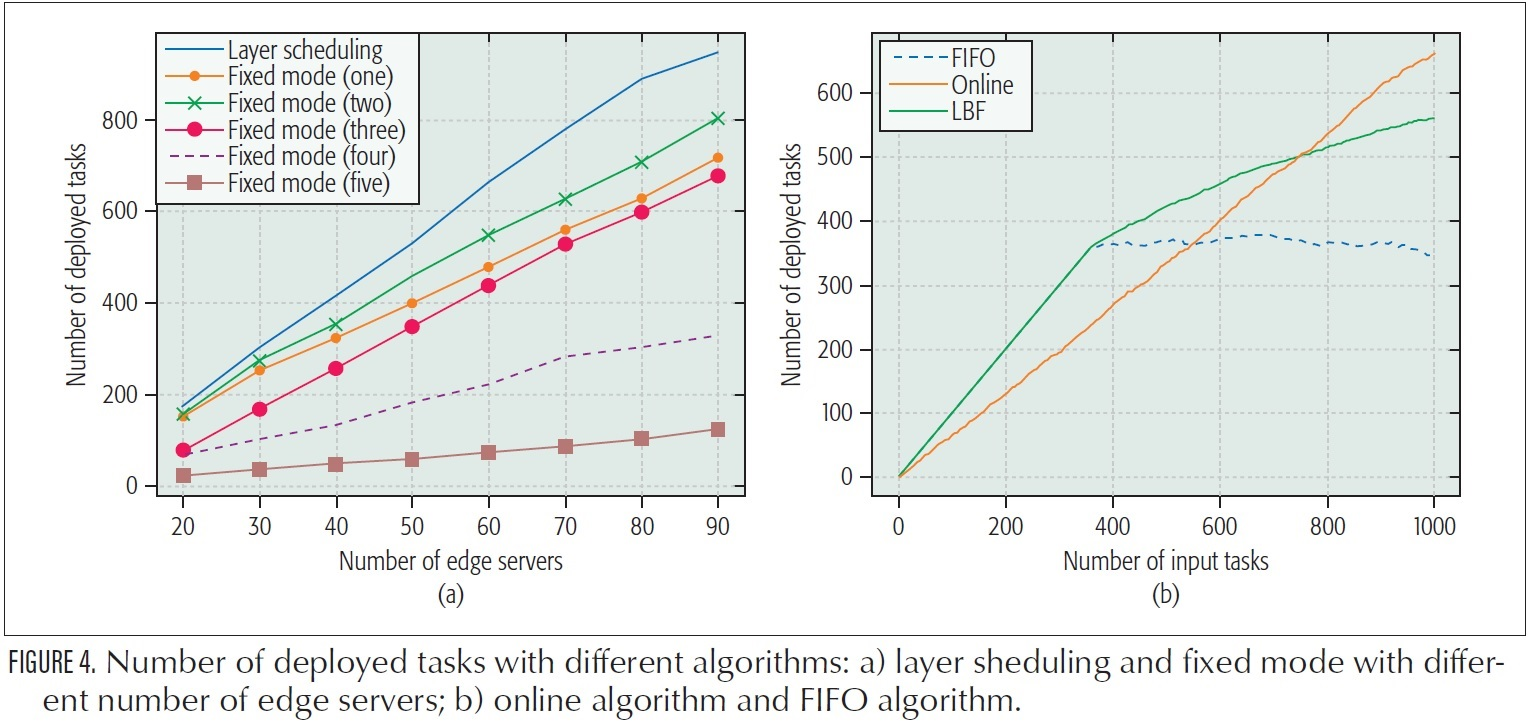
\includegraphics[width=1.12\linewidth]{Resources/Figura-4.jpg}
\end{figure}

%Vea la siguiente tabla:
%\begin{table}
%\vspace{2ex}
%\begin{tabular}{l l l}
%\toprule
%\textbf{Treatments} & \textbf{Response 1} & \textbf{Response 2}\\
%\midrule
%Treatment 1 & 0.0003262 & 0.562 \\
%Treatment 2 & 0.0015681 & 0.910 \\
%Treatment 3 & 0.0009271 & 0.296 \\
%\bottomrule
%\end{tabular}
%\caption{Table caption}
%\end{table}

\end{exampleblock}

%-------------------------------------------------------------------------------%

\end{column} % End of column 2.2

\end{columns} % End of the split of column 2

\end{column} % End of the second column

\begin{column}{\sepwid}\end{column} % Empty spacer column

\begin{column}{\onecolwid} % The third column

%-------------------------------------------------------------------------------%
%	CONCLUSION
%-------------------------------------------------------------------------------%

\begin{exampleblock}{Conclusion and Future Work}

We introduce deep learning for IoT into the edge computing environment to optimize network performance and protect user privacy in uploading data. The edge computing structure reduces the network traffic from IoT devices to cloud servers since edge nodes upload reduced intermediate data instead of input data. We propose algorithms to maximize the number of tasks in the edge computing environment. In the experiments, we choose 10 different CNN models as the deep learning networks and collect the intermediate data size and computational overhead from practical deep learning applications. The results of the performance evaluation show that our solutions can increase the number of tasks deployed in edge servers with guaranteed QoS requirements. As future work, we plan to deploy deep learning applications in a real-world edge computing environment with our algorithms.

\end{exampleblock}

%-------------------------------------------------------------------------------%
%	ADDITIONAL INFORMATION
%-------------------------------------------------------------------------------%

%\begin{exampleblock}{Additional Information}

%Info adicional. 
%\begin{itemize}
%\item Info 1.
%\item Info 2.
%\item Info 3.
%\end{itemize}

%\end{exampleblock}

%-------------------------------------------------------------------------------%
%	REFERENCES
%-------------------------------------------------------------------------------%

\begin{exampleblock}{References}

\nocite{*} % Insert publications even if they are not cited in the poster
\small{\bibliographystyle{unsrt}
\bibliography{referencias}\vspace{1cm}}
\end{exampleblock}

%-------------------------------------------------------------------------------%
%	ACKNOWLEDGEMENTS
%-------------------------------------------------------------------------------%

%\setbeamercolor{block title}{fg=red,bg=white} % Change the block title color

\begin{exampleblock}{Acknowledgements}

\small{\rmfamily{This work is supported by JSPS KAKENHI Grant Numbers JP16K00117, JP15K15976, and JP17K12669, the KDDI Foundation, and the Research Fund for Postdoctoral Program of Muroran Institute of Technology. Mianxiong Dong is the corresponding author.}} \\

\end{exampleblock}

%-------------------------------------------------------------------------------%
%	CONTACT INFORMATION
%-------------------------------------------------------------------------------%

%\setbeamercolor{block alerted title}{fg=black,bg=norange} % Change the alert block title colors
%\setbeamercolor{block alerted body}{fg=black,bg=white} % Change the alert block body colors

%\begin{block}{Contact Information}

%\begin{itemize}
%\item Web: \href{https://unis.edu.gt/}{https://unis.edu.gt/}
%\item Email: \href{mailto:info@unis.edu.gt}{info@unis.edu.gt}
%\end{itemize}

%\end{block}

%\begin{tabular}{rr}
%\hspace{0.3\linewidth} & %
\includegraphics[width=0.4\linewidth]{Resources/Logo_UNIS.png}
%\end{tabular}

%-------------------------------------------------------------------------------%

\end{column} % End of the third column

\begin{column}{\sepwid}\end{column} % Empty spacer column

\end{columns} % End of all the columns in the poster

\end{frame} % End of the enclosing frame
%\end{darkframes} % Uncomment for dark theme
\end{document}
